\clearpage
\section{Anexo}

\subsection{Comparativo Bases de Dados}
\label{anx:comparativo}

O DPVAT por muitos anos era uma responsabilidade da Seguradora Líder, mas a partir de 2021 teve administração instável, visto que Seguradora Líder foi dissolvida. Em 2023 a Caixa Econômica Federal torna-se responsável por gerenciar o DPVAT. Os dados do DPVAT sobre sinistros são divulgados em forma de relatório, sem que haja microdados para uma análise mais aprofundada. Enquanto sob a gestão da Seguradora Líder, havia anualmente um boletim estatístico\footnote{Disponível em \url{https://seguradoralider.com.br/Sala-de-Imprensa/Boletim-Estatistico}, acesso em 15/10/2023}, no qual há uma separação por unidade federativa, o que não é mais feito sob a gestão da Caixa -- encarregada pelos dados a partir de 2021.

\begin{table}[!ht]
    \centering
    \caption{Comparativo dados de óbitos para diferentes fontes no estado de São Paulo}
    \begin{tabular}{p{1.5cm}p{2cm}p{2cm}p{2cm}p{2cm}p{2cm}}
        Ano  & DPVAT & DATASUS & Infosiga & Infosiga* & Renaest \\ \hline
        2014 & 9.093 & 7.444 & ~ & ~ & ~ \\ \hline
        2015 & 6.884 & 6.270 & 6.493 & 6.168 & ~ \\ \hline
        2016 & 5.248 & 5.846 & 5.966 & 5.651 & ~ \\ \hline
        2017 & 6.103 & 5.462 & 5.649 & 5.350 & ~ \\ \hline
        2018 & 5.462 & 4.730 & 5.464 & 5.169 & 5.233 \\ \hline
        2019 & 6.026 & 5.181 & 5.422 & 5.123 & 5.164 \\ \hline
        2020 & 4.972 & 5.326 & 4.950 & 4.647 & 4.838 \\ \hline
        2021 & ~ & 5.416 & 4.925 & 4.649 & 4.847 \\ \hline
        2022 & ~ & 4.818 & 5.738 & 5.455 & 3.475 \\ \hline
    \end{tabular}
    \label{tab:comparativo}
    
    \vspace{2ex}
    
    {\raggedright * Removendo as rodovias federais}
    
\end{table}

Com base na Tabela \ref{tab:comparativo}, é possível observar as diferenças entre as bases de dados disponíveis e alguns detalhes merecem atenção. Primeiramente, é curioso que os números do DPVAT sejam maiores do que do Infosiga e Renaest, visto para ativar o seguro, é necessário entregar um Boletim de Ocorrência, que então constaria nessas bases. Uma possível explicação para essa inconsistência é de que o DPVAT é registrado quando o seguro é exercido, não quando ocorre o acidente, resultando em uma defasagem temporal.

Outro ponto que merece ser investigado é o fato de que em 2020 e 2021 os óbitos registrados pelo SUS superam os do Infosiga. Em teoria, todos os óbitos em decorrência de acidente de trânsito devem ser registrados no RDO (fonte de dados do Infosiga) para possibilitar o enterro da vítima, então se uma pessoa morreu no SUS, essa informação deveria estar disponível também no Infosiga. Portanto, os dados do DATASUS em teoria nunca deveriam superar os do Infosiga, principalmente se considerar que a vítima pode ser encaminhada para um hospital que não faz parte da rede SUS e, neste caso, seria contabilizado apenas no Infosiga.

Por fim, uma última inconsistência é observável no comparativo do Infosiga* com o Renaest. O Renaest não contabiliza sinistros em rodovias federais, então as BRs 381, 459, 101, 153, 116, 383, 158 e 488 foram removidas da base do Infosiga para fins de comparação. Como ambas as bases apresentam as mesmas fontes, os dados deveriam ser idênticos, mas nos anos de 2018 a 2021 há uma diferença de cerca de 500 óbitos. 

\clearpage
\subsection{Descrição base Renaest}
\label{anx:infosiga}

Tanto a base de dados do Infosiga quanto a do Renaest são alimentadas pela mesma fonte: os boletins de ocorrência da polícia. Entretanto, a forma como são divulgados é diferente, pelo Infosiga, de forma agregada em uma base de óbitos, no qual cada linha é uma vítima fatal, e uma base de não fatais, na qual cada linha é um acidente. É importante destacar que a forma como estes dados são agregados gera uma série de limitações, visto que com os microdados é possível investigar perguntas mais específicas e com maior profundidade.

Já a base disponibilizada pelo Renaest, apresenta um banco relacional, descrito na Figura \ref{fig:DERRenaest}, que apresenta dados menos agregados, mas ainda com limitações. Da forma como foram organizados os dados, se por exemplo uma motocicleta, um carro, um ônibus e um pedestre se envolvem em um sinistro, é possível saber se havia suspeita de álcool e quantas pessoas foram feridas. Entretanto, se houve uma fatalidade, não é possível saber em qual veículo essa vítima estava, bem como suas respectivas informações -- idade, gênero, se era motorista, se estava embriagada, etc. 

\begin{figure}[h]
    \centering
    \caption{Diagrama entidade relacionamento da base do Renaest}
    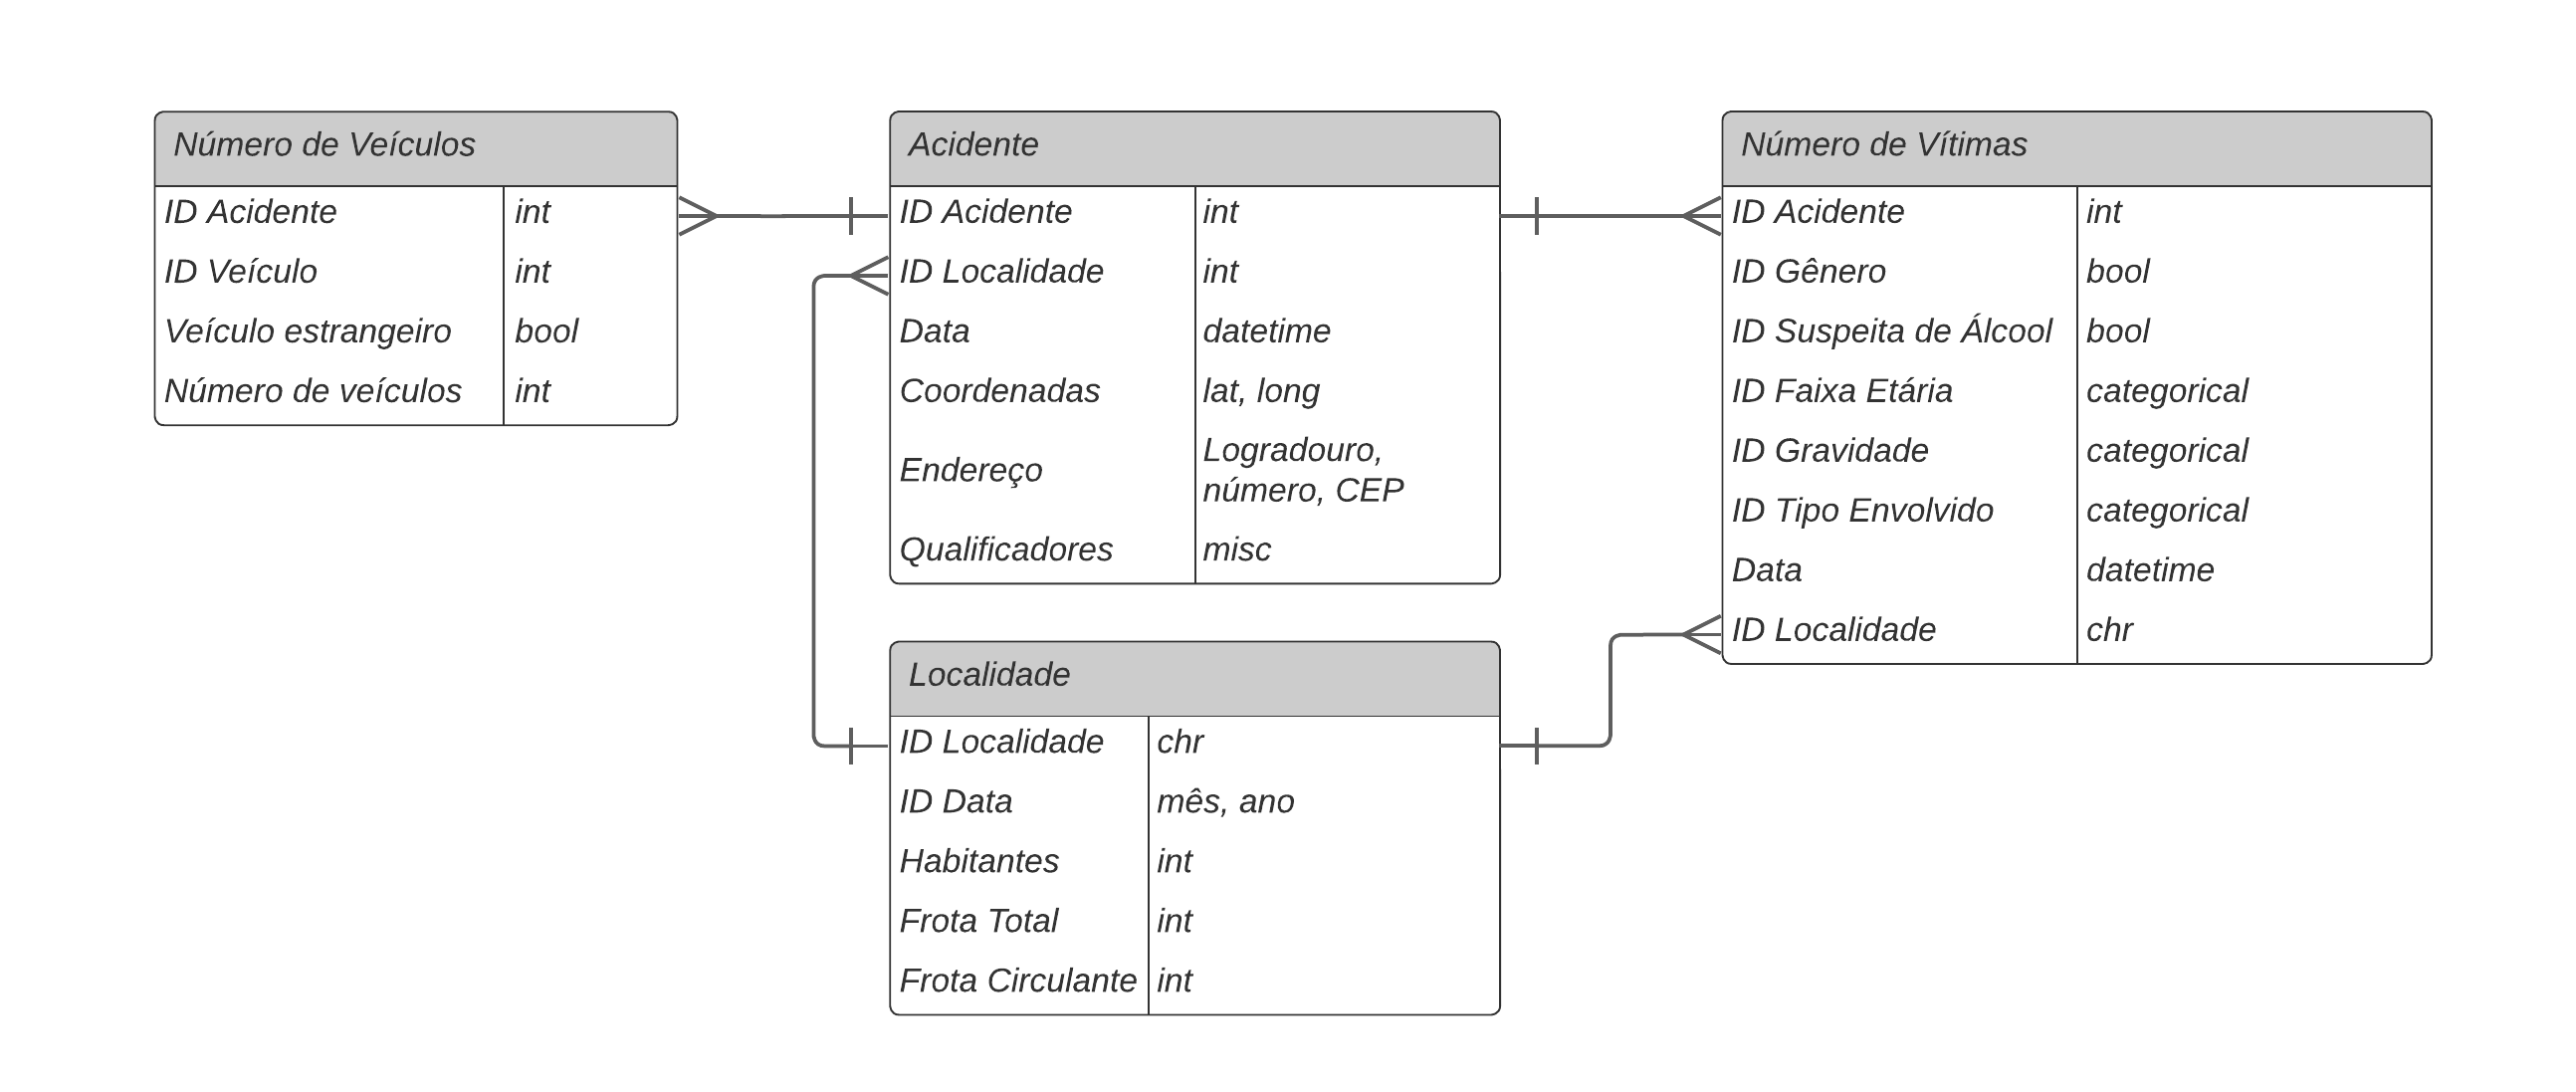
\includegraphics[width = 1\linewidth]{relatorios/faixa-azul/figuras/diagrama_base.png}
    \label{fig:DERRenaest}
\end{figure}

Considerando isso e a importância dessas informações para possíveis pesquisas dentro do universo da segurança viária, foi construído um diagrama (Figura \ref{fig:DERSug}) que contém uma proposta de como estes dados deveriam estar dispostos. Com a estrutura apresentada, os problemas apontados anteriormente não aconteceriam mais.

\begin{figure}[h]
    \centering
    \caption{Diagrama entidade relacionamento, sugestão para dados do Renaest}
    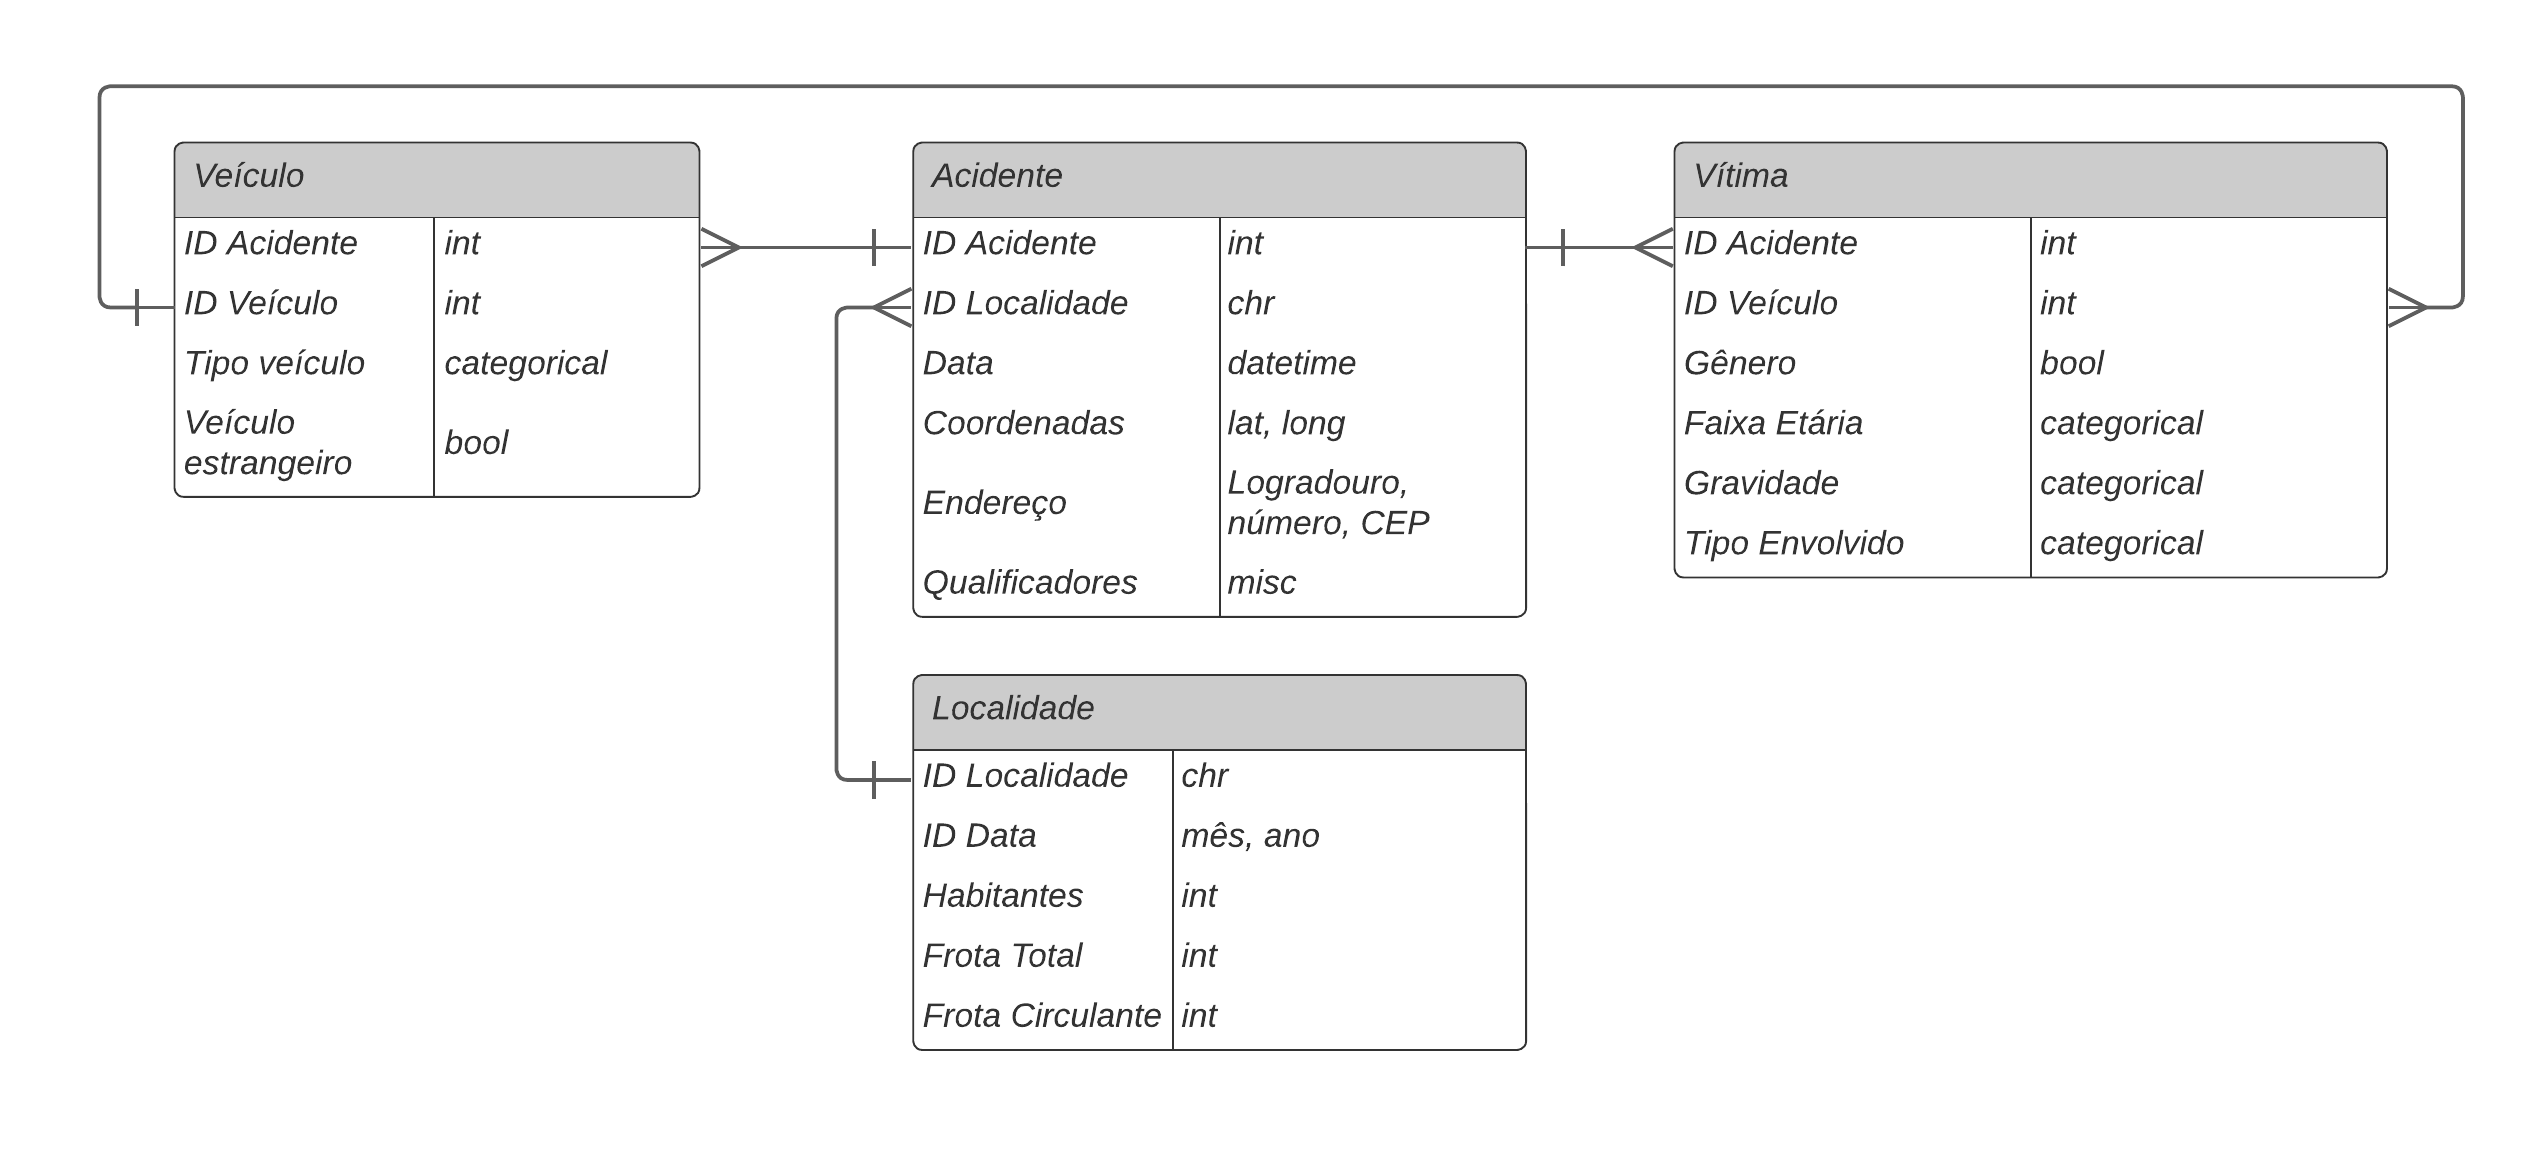
\includegraphics[width = 1\linewidth]{relatorios/faixa-azul/figuras/diagrama_sugestao.png}
    \label{fig:DERSug}
\end{figure}